\documentclass[a4paper, 12pt]{scrartcl}
\usepackage{ucs}
\usepackage[utf8x]{inputenc}
\usepackage[T1]{fontenc}
\usepackage[english,ngerman]{babel}
\usepackage{graphicx}
\usepackage{enumerate}
\usepackage{color}
\usepackage{amsfonts}
\usepackage{amsmath}
\usepackage{scrtime}
\usepackage[colorlinks=true,urlcolor=blue,linkcolor=black]{hyperref}


\begin{document}

\begin{normalsize}

\raggedright\textbf{\Huge Maschinelles Lernen}\\	
		\begin{flushright}
		Johannes Eifler und co\\
		Matrikel: 144915\\
		Stand: \space \today \space \thistime
		\end{flushright}

\end{normalsize}
%\piccaption{Enigma} 
%\parpic[l]{\includegraphics [width=0.6\linewidth]{enigma.jpg}}

\section*{lecture 1 (04.04.2016)}
\subsection*{Introduction}

	\begin{itemize}
	 \item supervised learning: learn relationships between variables
	 \item unsupervised learning: learn some structure of measured variables
	\end{itemize}
	
	\\
	Dependend variables are measured at independant variables (covariates). Variables are measured on some \textbf{scale}:
	\\
	
	\begin{itemize}
	 \item nominal (gender, color)
	 \item ordinal (ranking of soccerteams)
	 \item interval (temperature in degree celsius)
	 \item rational (temperature in kelvin, weight, height), has meaningful zero in comparison to interval
	\end{itemize}
	
	$\Rightarrow$ quotients make sense on ratio scale; quotiens of differences make sense on interval scale\\
	
	metric scale: interval- and ratio scale  \\

\subsection*{problems in machine learning:}

	\begin{enumerate}[1.]
	 \item \textbf{regression}: one dependent variable on \textcolor{red}{metric scale}\\
	 one or more independent variables on \textcolor{red}{metric scale}
	 \item \textbf{variance analysis}: one dependent variable on \textcolor{red}{metric scale}\\
	 one or more independent variables on \textcolor{red}{nominal scale}
	 \item \textbf{classification}: one dependent variable on \textcolor{red}{nominal scale}\\
	 one or more independent variables on \textcolor{red}{metric scale}
	 \item \textbf{contingency analysis}: one dependent variable on \textcolor{red}{nominal scale}\\
	 one or more independent variables on \textcolor{red}{nominal scale}
	 \item \textbf{scaling problems}: independent variables on \textcolor{red}{arbitrary scale} but measurements on ordinal scale\\
	 dependent variables on \textcolor{red}{metric scale}
	\end{enumerate}

\subsection*{linear regression}

	data/measurements: $(x^{(1)}, y^{(1)}), \dots , (x^{(n)}, y^{(n)})$ \\\\
	$x^{(i)}$ independent/covariates $\in \mathbb{R}^n$ ($n$ - variables)\\
	$y^{(i)}$ dependent/variates $\in \mathbb{R}^n$\\
	%includegraphics{graphs/plot.eps} \\
	plot suggests a linear dependence between $x$ and $y$ \\
	$y = \Theta_1 x + \Theta_0$\\\\
	in the multivate case: $y = \Theta_0 + \Theta_1 X_1 + \dots + \Theta_n X_n$\\
	$= \Theta^T X, X = (1, X_1, \dots ,X_n ) \in \mathbb{R}^{n+1}$\\\\
	
	%TODO Ich glaube hier ff. wurden irgendwie die m und n vertauscht -Sascha
	 problem: estimate the parameter vector $\Theta \in \mathbb{R}^{n+1}$ from the measurements $(x^{(1)}, y^{(1)}), \dots , (x^{(n)}, y^{(n)})$\\
	loss function: $\textcolor{red}{L(\Theta)} = \frac{1}{2} \Sigma^m_{i=1} (\Theta^T X^{(i)} - y^{(i)})^2$\\
	\textcolor{red}{model loss $\hat{=}$ loss for parameter vector $\Theta$}\\\\
	goal: choose $\Theta \in \mathbb{R}^{n+1}$ that minimizes the loss function\\
	reformulation:\\\\
	data matrix:
	%TODO Möglicherweise müssten hier die x ab x^0  zählen -Sascha
	\[ X =\left( \begin{array}{ccc}
	x^{(1)^T} \\
	\vdots \\
	x^{(n)^T} \end{array} \right) \in \mathbb{R}^{m \times (n+1)}\]
	response vector:
	
	\[ Y =\left( \begin{array}{ccc}
	y^{(1)} \\
	\vdots \\
	y^{(n)} \end{array} \right) \in \mathbb{R}^n\]
	parameter vector:
	
	\[ \Theta =\left( \begin{array}{ccc}
	\Theta_0 \\
	\vdots \\
	\Theta_n \end{array} \right) \in \mathbb{R}^{n+1}\]

	loss function in vectorized form:
	\[L(\Theta) = \frac{1}{2} \Sigma^m_{i=1} (\Theta^T * X^{(i)} - Y^{(i)})^2 = \frac{1}{2} \lVert \textcolor{red}{X * \Theta} - \textcolor{blue}{Y} \lVert^2_2\]
	
	\begin{center}
	( \textcolor{red}{vector of predictions}$\quad\quad\quad$ \textcolor{blue}{vector of observation response} )
	\end{center}
	\[ = \frac{1}{2} (X * \Theta -Y)^T * (X * \Theta - Y)\]
	\begin{center}
	(definition of the euclidian norm)
	\end{center}
	\[ = \frac{1}{2} (\Theta^T X^T \times \Theta - \textcolor{red}{\Theta^T X^T Y - Y^T X*\Theta} + Y^T Y)\]
	\begin{center}
	= $-2 \Theta^T X^T Y$ since the dot product is symmetric ($X^T Y = Y^T X$)
	\end{center}
	\[= \frac{1}{2} \Theta^T X^T X \Theta - \Theta^T X^T Y + \frac{1}{2} Y^T Y\]
	remember from calculus: A neccessary condition for an optimum of the (loss-) function is that the gradient vanishes.\\
	
	$\bigtriangledown_{\Theta} L(\Theta) \stackrel{!}{=} 0 \quad\quad\quad\quad\quad\quad\quad\quad\quad  t(x) = \frac{1}{2}x^2+ax+b$\\
	$\bigtriangledown_{\Theta} L(\Theta) = X^T X \Theta * X^T Y \stackrel{!}{=} 0  \quad\quad\quad \bigtriangledown_x t(x) = x+a$\\\\
	here we have used that $X^T X$ is symmetric\\\\
	$\Rightarrow X^T X \Theta = X^T Y \quad\quad\quad\quad\quad t(\Theta) = \Theta^T X \Theta$\\
	$\Rightarrow  \Theta = (X^T X)^{-1} X^T Y \quad\quad\quad\quad\quad \bigtriangledown_{\Theta} t(\Theta) = (X+X^T)\Theta$\\
	privided that $(X^T X)^{-1}$ exists\\\\
	$\textcolor{red}{(X^T X)_{ij}} = X^{(i)^T}X^{(j)}$\\
	\textcolor{red}{operation matrix}\\
	dot product of i-th dataa point and j-th data point\\\\
	hence, the last square solution of the linear regression problem is $\Theta = (X^T X)^{-1} X^T Y$\\\\
	more robust solution:\\\\
	$\Theta = (X^T X + \gamma \mathds{1})^{-1} X^T Y, \quad\quad \gamma > 0$ regularization parameter\\\\
	ridge regression solution is not only more robust numerically, but also statistically (it is not so sensitive to small measurement errors in $X$).\\\\
	Natural question: which loss function gives us the ridge regression solution?\\\\
	answer: $\quad\quad L_{ridge} (\Theta)= \textcolor{red}{\frac{1}{2} \lVert X * \Theta - Y \lVert_2^2} + \textcolor{blue}{\gamma \lVert \Theta \lVert_2^2}$
	\begin{center}
	\textcolor{red}{loss term} \space\space \textcolor{blue}{reularisation term}
	\end{center}
	probabilistic interpretation of least squares
	\[ Y = \textcolor{red}{\Theta^T * X} + \textcolor{blue}{\epsilon} \]
	\begin{center}
	\textcolor{red}{deterministic part} \space\space \textcolor{blue}{random/noise part}
	\end{center}
	model of the noise: gaussian noise \space\space $p(\epsilon)= \frac{1}{\sqrt{2\pi}\sigma} \exp (- \frac{\epsilon^2}{2 \sigma^2}) \quad$ (probability density function)\\
	$P[a \leq \epsilon \leq b] = \int_a^b p(\epsilon)\quad d\epsilon$\\\\
	$Y$ is a function of the random noise term $\epsilon$ als a random variable. The probability density function of $Y$ is:
	\[ p(Y) = \frac{1}{\sqrt{2 \pi}\sigma} \exp(- \frac{\lVert Y - \Theta^T X \lVert^2_2}{2 \sigma^2})\]

\section*{lecture 2 (06.04.2016)}
\subsection*{linear regression}
data: \space \[(x^{(1)}, y^{(1)}), \dots , (x^{n}, y^{n})\]
\[x^{(i)} \in \mathbb{R}^n \quad\quad covariates\]
\[y^{(i)} \in \mathbb{R} \quad\quad variates/response \]
assumption:
\begin{enumerate}[(1)]
\item $y = t(x) \quad\quad y$ is function of $x$\\
linear regression \space\space \framebox{$y = \textcolor{red}{\Theta^T} x$} \space $\Theta \in \mathbb{R}^{n+1}$ (parameter vector)\\
\textcolor{red}{\quad\quad\quad\quad\quad\quad\quad\quad\quad$\Sigma^n_{i = 0} \Theta_i x_i$}\\
$x= (1,x_1, \dots ,x_n) \in \mathbb{R}^{n+1} \quad \quad x_0 = 1$
\item data are obscured by random noise:\\\\
$y = \Theta^T x +\epsilon, \quad\quad \epsilon = $ random noise term\\
$p(\epsilon) = \frac{1}{\sqrt{2\pi}} r \exp (- \frac{\epsilon^2}{2 \sigma^2})$\\

%TODO Hier einen entsprechenden Graphen einfügen
	\begin{figure}
		\centering
		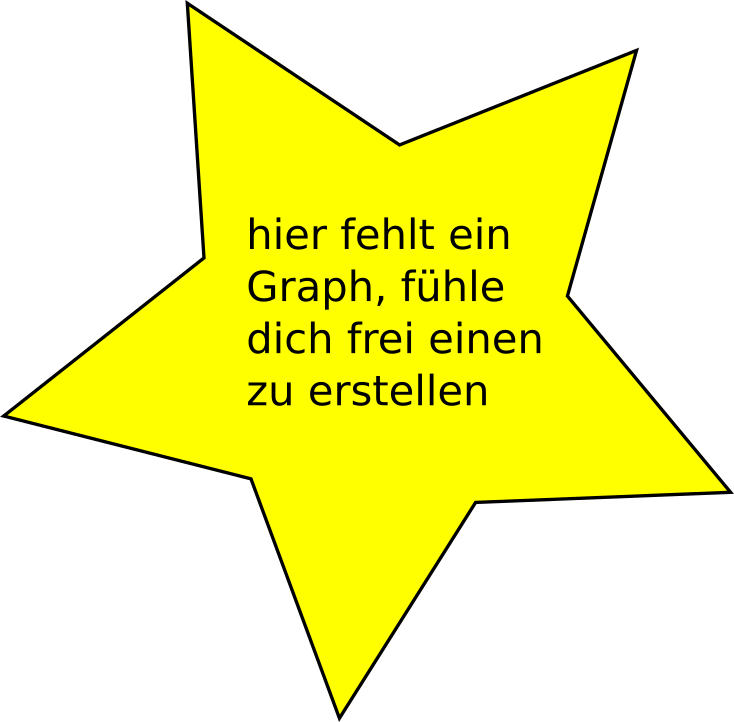
\includegraphics[width=0.7\linewidth]{graphs/dummy}
		%includegraphics{graphs/plot2.eps} \\
	\end{figure}

since $\epsilon$ is random, also $y$ is random with density $p(y|x, \Theta) - \frac{1}{\sqrt{2\pi}r} \exp (- \frac{\lVert y- \Theta^T x\lVert^2}{2r^2})$\\
To specify the model we have to estimate $\Theta \in \mathbb{R}^{n+1}$ from the data\\\\
idea: choose $\Theta$ that maximizes the likelihood\\\\
likelihood function:
\[L(\Theta) = \prod^m_{i=1} p(y^{(i)}|x^{(i)};\Theta)\]
the product form means: the observation $(x^{(1)},y^{(1)}), \dots , (x^{(i)}, y^{(i)})$ are independent of each other\\\\
estimate:
\[ \Theta_{ML} = \underset{\Theta \in \mathbb{R}^{n+1}}{argmax} L(\Theta) \]
\[ = \underset{\Theta \in \mathbb{R}^{n+1}}{argmax} \prod^m_{i=1} \frac{1}{\sqrt{2 \pi} \sigma} \exp \left(- \frac{(y^{(i)} - \Theta^T x^{(i)})^2}{2 \sigma^2}\right)\]
since we are only interested in the positoin where the maximum is attained we can apply a monoton transformation to $L(\Theta)$ with changing this position\\\\
$\Rightarrow \log$-likelihood function: $l(\Theta) = \log L(\Theta)$
\[ = \Theta_{ML} = \underset{\Theta \in \mathbb{R}^{n+1}}{argmax} l(\Theta)\]
\[ = \underset{\Theta \in \mathbb{R}^{n+1}}{argmax} \Sigma^m_{i=1} - \log (\sqrt{2\pi}\sigma) - \frac{1}{2\sigma}(y^{(i)} - \Theta^T x^{(i)})^2\]
\[\underset{\Theta \in \mathbb{R}^{n+1}}{argmax} - \textcolor{red}{m \log (\sqrt{2\pi}\sigma)} - \frac{1}{2\textcolor{blue}{\sigma^2}}\Sigma^m_{i=1}(y^{(i)} - \Theta^T x^{(i)})^2  \]
\begin{center}
\textcolor{red}{does not depend on $\Theta$}\space\space\space \textcolor{blue}{scaling vector does not influence the optimal $\Theta$}
\end{center}
\[ \underset{\Theta \in \mathbb{R}^{n+1}}{argmax} -\frac{1}{2} \Sigma^m_{i=1}(y^{(i)}-\Theta x^{(i)})^2\]
$X$: data matrix\\
$\Theta$: parameter vector\\
$Y$: response vector
\[\underset{\Theta \in \mathbb{R}^{n+1}}{argmax} -\frac{1}{2} \lVert X * \Theta - Y \lVert^2_2\]
\[ \underset{\Theta \in \mathbb{R}^{n+1}}{argmax} \textcolor{red}{\frac{1}{2} \lVert X * \Theta - Y \lVert^2_2}\]
\begin{center}
\textcolor{red}{$L(\Theta)$ loss function}\\
Minimizing the loss function that we discussed already\\
\end{center}
\end{enumerate}
\subsection*{remark} going non-linear $x \in \mathbb{R}, y \in \mathbb{R} \quad y=t(x)$
\begin{addmargin}[2 cm]{0 cm}
observations: $(x^{(1)}, y^{(1)}), \dots ,(x^{(i)}, y^{(i)}) \in \mathbb{R} \times \mathbb{R}$ but $f(.)$ not neccessarily linear function\\\\
$((x^{(1)},x^{(1)^2}, x^{(1)^3}), y^{(1)}), \dots , ((x^{(m)},x^{(m)^2}, x^{(m)^3}), y^{(m)})$\\
apply linear regression to argumented data points:\\\\
$\Rightarrow y = \Theta_0 + \Theta_1  x + \Theta_2  x^2 + \Theta_3 x^3$\\\\
linear regression gives \glqq good estimates\grqq\ for $\Theta_0, \Theta_1, \Theta_2, \Theta_3$\\\\
overfitting problem!

%TODO Hier einen entsprechenden Graphen einfügen
	\begin{figure}
		\centering
		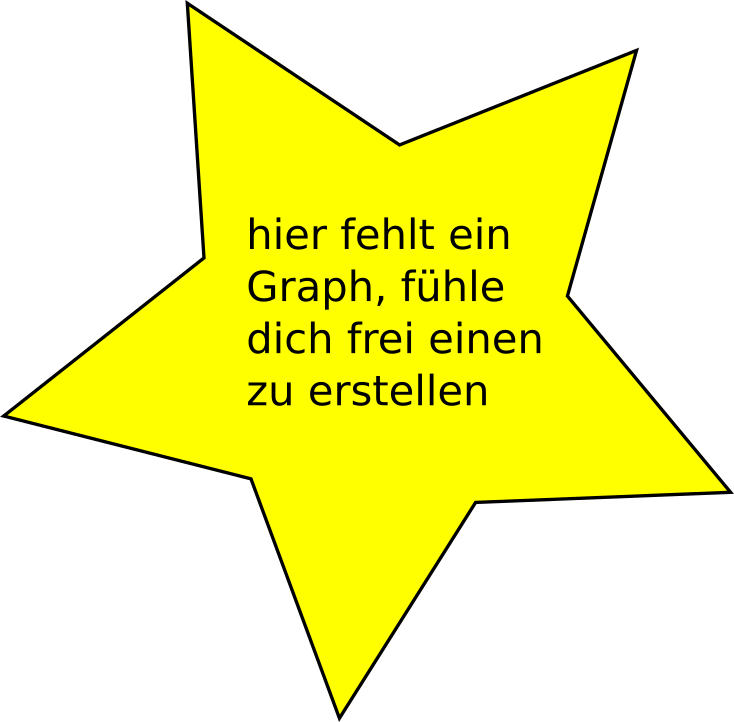
\includegraphics[width=0.7\linewidth]{graphs/dummy}
		%includegraphics{graphs/plot3.eps} \\
	\end{figure}
	
\end{addmargin}

\subsection*{logistic regression for binary classification}
data/observations: $(x^{(1)}, y^{(1)}), \dots , (x^{(i)}, y^{(i)})$\\\\
\begin{center}
 $x^{(i)} \in \mathbb{R}^n$ \space covariates\\
 $y^{(i)} \in {0,1}$ \space variates/response
\end{center}
probabilistic model of logistic regression
\[P[y=1|x;\Theta] = h_{\Theta}(x) \in (0,1)\]
\[P[y=0|x;\Theta] = 1-h_{\Theta}(x) \]

$h_{\Theta}(x) = g(\Theta^T x)$, where $g(.)$ is the logistic function $g(z) = \frac{1}{1+\exp(-z)}$\\\\
goal(as in linear regression): estimate $\Theta \in \mathbb{R}^n$ (Parameter vector) from data.\\
likelihood function for parameter vector $\Theta$:
\[L(\Theta) = \prod^m_{i=1} P[y^{(i)}|x^{(i)} ; \Theta]\]
again, assumption of independent observation
\[= \prod^m_{i=1} \textcolor{red}{h_{\Theta}(x^{(i)})^{y^{(i)}}} \textcolor{blue}{(1-h_{\Theta}(x^{(i)}))^{1-y^{(i)}}}\]
\begin{center}

$\textcolor{red}{=\begin{cases}1&\text{if $y^{(i)} = 0$}\\h_{\Theta}(x^{(i)})&\text{if $y^{(i)} = 1$}\end{cases}}$
$\textcolor{blue}{=\begin{cases}1&\text{if $y^{(i)} = 1$}\\1-h_{\Theta}(x^{(i)})&\text{if $y^{(i)} = 0$}\end{cases}}$\\
$\textcolor{red}{h_{\Theta} := P[y^{(i)} = 1 | x^{(i)};\Theta]}$\space\space
$\textcolor{blue}{1-h_{\Theta}(x^{(i)}) := P[y^{(i)} = 0 | x^{(i)};\Theta]}$
\end{center}

instead of working with the likelihood function it is easier to work with the $\log$-likelihood function:
\[\Theta_{ML} = \stackrel{argmax}{\Theta \in \mathbb{R}^n} L(\Theta) = \stackrel{argmax}{\Theta \in \mathbb{R}^n} \log \underbrace{L(\Theta)}_{\substack{l(\Theta)}}\]
\[= \stackrel{argmax}{\Theta \in \mathbb{R}^n} \Sigma^m_{i=1} y^{(i)} \log h_{\Theta}(x^{(i)}) + \underbrace{(1-y^{(i)}) \log(1-h_{\Theta}(x^{(i)}))}_{\substack{\log \text{likelihood function}}}\]
neccessary for optimum is a vanishing gradient\\
$\bigtriangledown_{\Theta} l(\Theta) \stackrel{!}{=}0$\\
for computing the gradient:
\[\frac{d}{dz} g(z) = \frac{d}{dz} \frac{1}{1+\exp(-z)}\]
\[= \frac{\exp(-z)}{(1+ \exp (-z))^2}\]
\[= \frac{1}{1+\exp (-z)} (\frac{1+\exp(-z) -1}{1+\exp(-z)})\]
\[= \frac{1}{1+\exp(-z)} (1-\frac{1}{1+\exp(-z)})\]
\[= \framebox{g(z)(1-g(z))}\]
\newline
\[\bigtriangledown_{\Theta} l(\Theta) = (\frac{\delta}{\delta \Theta_1} l(\Theta), \dots , \frac{\delta}{\delta \Theta_1} l(\Theta))\]
\[\frac{\delta}{\delta \Theta_j} l(\Theta)= \frac{\delta}{\delta \Theta_j} \Sigma^m_{i=1} y^{(i)}\log h_\Theta(x^{(i)}) + (1-y^{(i)}) \log (1-h_\Theta(x^{(i)}))\]
\[= \Sigma^m_{i=1} \left( \frac{y^{(i)}}{h_\Theta(x^{(i)})} - \frac{1-y^{(i)}}{1-h_\Theta(x^{(i)})}\right) \frac{\delta}{\delta\Theta_j} \underbrace{h_\Theta(x^{(i)})}_{\substack{g(\Theta^Tx^{(i)})}}\]
\[=\Sigma^m_{i=1} \left( \frac{y^{(i)}}{h_\Theta(x^{(i)})} - \frac{1-y^{(i)}}{1-h_\Theta(x^{(i)})}\right)\]
\[h_\Theta(x^{(i)})(1-h_\Theta(x^{(i)}))\underbrace{x^{(i)}_j}_{\substack{\text{j-th component i-th data vetor}}}\]
\[= \Sigma^m_{i=1} y^{(i)}(1-h_\Theta(x^{(i)}))-(1-y^{(i)})h_\Theta(x^{(i)})x^{(i)}_j\]
\[= \Sigma^m_{i=1}( y^{(i)}-h_\Theta(x^{(i)}))x^{(i)}_j\]
Unfortunetaly the system of equations $\frac{\delta}{\delta\Theta_j} l(\Theta)\stackrel{!}{=}0$ is highly non-linear and thus difficult to solve!
\[= \Sigma^m_{i=1}( y^{(i)}-h_\Theta(x^{(i)}))x^{(i)}_j = 0\]
turn to a numerical scheme(gradient ascend):\\\\
initialize: $\Theta^{(0)}$ arbitrary with some vector in $\mathbb{R}^n$\\
repeat
\begin{addmargin}[2 cm]{0 cm}
for $i=1$ to $m$
\begin{addmargin}[2 cm]{0 cm}
$\Theta_j^{(k)} = \Theta^{(k-1)}_j + \underbrace{\alpha}_{\substack{learning rate}} \Sigma^m_{i=1}(y^{(i)} - h_{\Theta^{(k)}} x^{(i)})x_j^{(i)}$
\end{addmargin}
end for
\end{addmargin}
until convergence
%bild

\section*{lecture 3 (11.04.2016)}
\subsection*{differentiability and convexiability}

Differentiability: function $t: \mathbb{R}^n \rightarrow \mathbb{R}, x \mapsto t(x)$\\
$t$ is differentiable at $x \in \mathbb{R}^n$ if $t$ can approximated well in x by a linear function.
\[\exists t'(x): t(y) = t(x) + \textcolor{red}{t'(x)^T} (y-x) + \textcolor{blue}{o(\lVert y-x\lVert)}\]
\begin{center}
\textcolor{red}{$\in \mathbb{R}^n$}\space\space\textcolor{blue}{little o-notation $\stackrel{lim}{r \rightarrow 0} \frac{1}{r} o(r) = 0$} 
\end{center}
not always possible:
%bild1
\subsection*{the gradient $t'(x)$ in coordinates}
using the definition of differentiability we can plug in special values for $y$.
\[y^{(i)}(t) = x + t\textcolor{red}{e_i}\]
\begin{center}
 \textcolor{red}{i-th standard basis vector $e_i = (0, \dots, 0,1,0, \dots ,0)^T, o(0)=0$ (the $1$ is position $i$)}
\end{center}
by differentiability we have:
\[t(y^{(i)}(t)) = t(x) + t'(x)^Ty^{(i)}(t) + o(\lVert y^{(i)}(t)-x\lVert)\]
\[= t(x) + tt'(x)^Te_i+o(t)\]
\[\Rightarrow t(y^{(i)}(t)) - t(x) - tt'(x)^Te_i = o(t)\]
\[\Rightarrow \frac{t(y^{(i)}(t))}{} - t'(x)^{T}e_i = \frac{1}{t} o(t)\]
\[\Rightarrow \textcolor{red}{\stackrel{lim}{t \rightarrow 0} \frac{t(y^{(i)}(t))}{t}} = \textcolor{blue}{t'(x)^Te_i}\]
\begin{center}
 \textcolor{red}{$= \frac{\delta t}{\delta x_i}(x)$ partial derivative}\space\space\textcolor{blue}{i-th component of the vector $t'(x)$ (gradient)}
\end{center}
\[\Rightarrow t'(x) = (\frac{\delta t}{\delta x_1}, \dots , \frac{\delta t}{\delta < n}(x))\]
generalization to functions $t: \mathbb{R}^n \rightarrow \mathbb{R}^m$\\
$t$ is called differentiable in $x \in \mathbb{R}^n$ if $\exists t'(x)\in\mathbb{R}^{m \times n} sit \forall y \in \mathbb{R}: t(y):$
\[ \underbrace{t(x)+t'(x)(y-x)}_{\substack{\text{linear approx.}}}+\underbrace{(|y-x|)}_{\substack{\text{vector little o-notation}}}\] 
here  $t'(x)$ is called Jacobi-Matrix\\\\

in coordinates:

\[ t'(x) =\left( \begin{array}{ccc}
\frac{\delta t_1}{\delta x_1} \dots  \frac{\delta t_1}{\delta x_n}\\
\vdots \quad \quad \quad \vdots\\
\frac{\delta t_m}{\delta x_1} \dots  \frac{\delta t_m}{\delta x_n} \end{array} \right)\] 


\[\lim_{v \rightarrow 0} \frac{1}{\lVert v \lVert} \quad o(v) = o \in \mathbb{R}^m \]
\[o(\underbrace{0}_{\substack{\in \mathbb{R}^m}})= 0\]
special case: assume, that $t: \mathbb{R}^n \rightarrow \mathbb{R}$ is differentiable in every $x \in \mathbb{R}^n$. That means $t'(x)$ exists for every $x \in \mathbb{R}^n$! Use this to define a new function:
\[t': \mathbb{R}^n \rightarrow \mathbb{R}^n , x \mapsto t'(x)\]
in coordiantes:

\[ t'(x) =\left( \begin{array}{ccc}
\frac{\delta^2 t}{\delta x_1 \delta_{x_1}}(x) \dots  \frac{\delta^2 t}{\delta x_n \delta_{x_1}}(x)\\
\vdots \quad \quad \quad \vdots\\
\frac{\delta^2 t}{\delta x_1 \delta_{x_n}}(x) \dots  \frac{\delta^2 t}{\delta x_n \delta_{x_n}}(x) \end{array} \right)\]

\subsection*{convex functions}
a subset $K \subset \mathbb{R}^n$ is called convex, if every $p,q \in K$ also $\lambda p + (1-\lambda) q \in K$ for $\lambda \in [0,1]$\\

%pic

a function $t:\mathbb{R}^n \rightarrow \mathbb{R}$ is called convex, if the epi-graph of the function 
\[epi(t) = \{(x,y) \in \mathbb{R}^{n+1} | y \geq f(x)\}\]
is a convex set

%pic

alternative characterization of convexity of functions:\\
$t: \mathbb{R}^n \rightarrow \mathbb{R}$ is convex, if for all $x,y \in \mathbb{R}^n$:
\[t(\lambda x + (1-\lambda)y) \leq \lambda t(x) + (1-\lambda) + t(x)\]

%pic
\begin{framed}
lemma: a differentiable function $t: \mathbb{R} \rightarrow \mathbb{R}$ is convex if and only if $t':\mathbb{R} \rightarrow \mathbb{R}$ ($x \mapsto t'(x)$) is increasing
\end{framed}

that is, it is enough to look at point $p,q \in \mathbb{R}^{n+1}$ that we on the boundary of the epi-graph of $t$

%proof

\begin{framed}
corrollary: a twice differentiable function is convex if its second derivative is always non-negative.\\
follows from: a differential function $t: \mathbb{R} \rightarrow \mathbb{R}$ is increasing if its derivative is non-negative
\end{framed}

\begin{framed}
theorem: a twice differential function $t: \mathbb{R}^n \rightarrow \mathbb{R}$ is convex, if and only if the hessian os positive semi-definite.

%proof
\end{framed}


\end{document}